\documentclass[10pt,a4paper]{article}

\usepackage[margin=2.2cm]{geometry}
\usepackage[T1]{fontenc}
\usepackage[utf8]{inputenc}
\usepackage{lmodern}
\usepackage{microtype}
\usepackage{amsmath}
\usepackage{graphicx}
\usepackage{booktabs}
\usepackage{listings}
\usepackage{xcolor}
\usepackage{tikz}
\usetikzlibrary{arrows.meta,positioning,shapes.geometric,fit,calc}
\usepackage[hidelinks]{hyperref}

% compact lists without enumitem
\let\olditemize\itemize
\renewcommand{\itemize}{\olditemize\setlength{\itemsep}{1pt}\setlength{\topsep}{2pt}\setlength{\parsep}{0pt}}
\let\oldenumerate\enumerate
\renewcommand{\enumerate}{\oldenumerate\setlength{\itemsep}{1pt}\setlength{\topsep}{2pt}\setlength{\parsep}{0pt}}

\lstset{
  basicstyle=\ttfamily\footnotesize,
  breaklines=true,
  frame=single,
  framerule=0.2pt,
  showstringspaces=false,
  keywordstyle=\bfseries,
  commentstyle=\color{gray},
}

\title{\textbf{Deliveroo Autonomous Agent}\\[2pt]
\large Project Report --- Autonomous Software Agents, A.A. 2025--2026}
\author{
  Matteo Ranzi\thanks{Matricola: 209449, Email: \texttt{matteo.ranzi@studenti.unitn.it}}
  \and
  Luca Hardonk\thanks{Matricola: 267750, Email: \texttt{luca.hardonk@studenti.unitn.it}}
}
\date{September 2026\\[4pt]
\small Repository: \url{https://github.com/matteoranzi/Autonomous-Software-Agent---Deliveroo.js}}

\begin{document}
\maketitle

\section{Introduction}

This report documents the design and implementation of a team of autonomous software agents for
the Deliveroo.js game, in which agents move on a grid map, pick up parcels whose reward decays
over time, and deliver them to dedicated delivery tiles. The project comprises:

\begin{itemize}
    \item \textbf{Agent A}, a Belief--Desire--Intention~\cite{bratman1987} agent written in
    TypeScript, designed in the spirit of practical, modular BDI
    implementations~\cite{caillou2015,traldi2022}, whose
    distinguishing features are (i) an event-driven belief-revision layer built on pluggable
    change-detection strategies, (ii) intention selection performed by a Monte Carlo Tree Search
    (MCTS) over a dynamically built, logical (desire-level) state-space graph, (iii) a
    Mamdani-style fuzzy inference system used as the common reward signal that makes
    heterogeneous metrics (cost, reward, urgency) comparable, and (iv) a layered planning stack
    combining A* pathfinding with an \emph{anytime} PDDL planner able to push crates out of the
    way (Sokoban-style), obtained by extending the open-source Planning-as-a-Service (PaaS)
    infrastructure.
    \item \textbf{Agent B}, an LLM-controlled agent that translates natural-language requests
    into structured, bounded plans executed through a constrained interpreter, and that can drive
    a second agent through a typed Model Context Protocol (MCP) interface.
\end{itemize}

The report follows the structure of the agent itself: beliefs
(Section~\ref{sec:beliefs}), desires (Section~\ref{sec:desires}), intentions and MCTS
(Section~\ref{sec:intentions}), fuzzy scoring (Section~\ref{sec:fuzzy}), planning and PDDL
(Section~\ref{sec:planning}), the LLM agent (Section~\ref{sec:llm}), and validation
(Section~\ref{sec:validation}).

\section{Architectural Design}
\label{sec:architecture}

The BDI agent is organised as a pipeline of loosely coupled components, each behind an interface
so that alternative implementations can be swapped without touching the deliberation loop
(Figure~\ref{fig:architecture}). Raw socket payloads from the Deliveroo.js server are first
normalised by a thin \emph{adapter} layer (\texttt{io/adapters/}) into internal types, decoupling
the belief base from the wire format. The \texttt{Belief} object is the single source of truth;
every downstream component (desire generation, intention selection, cost estimation, planning)
reads from it and never from the network directly.

\begin{figure}[htbp]
\centering
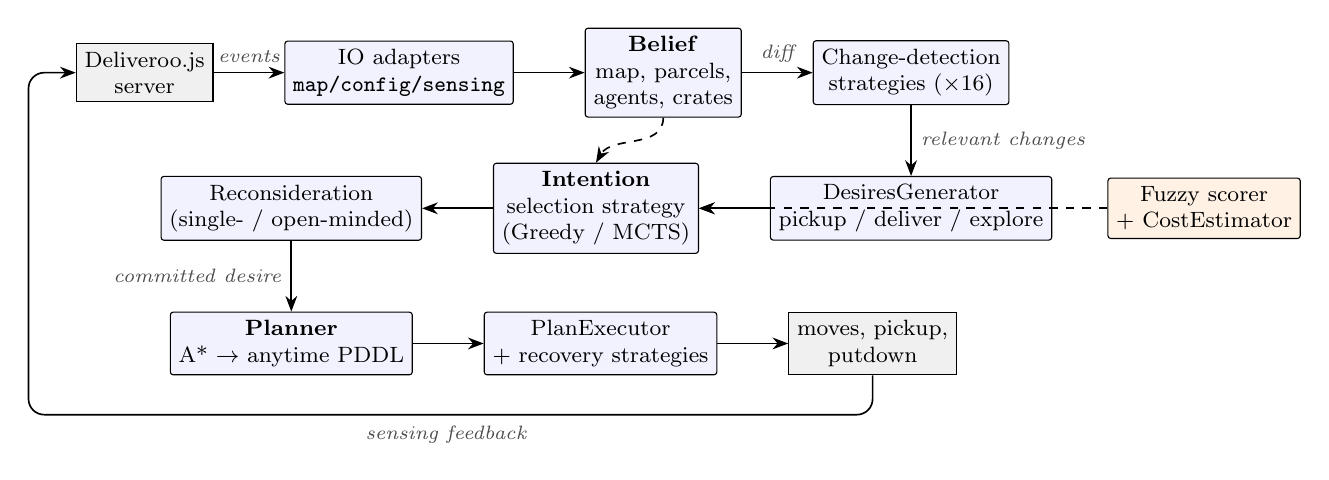
\begin{tikzpicture}[
    font=\footnotesize,
    node distance=5mm and 9mm,
    box/.style={draw, rounded corners=1pt, align=center, minimum height=7mm, inner sep=3pt, fill=blue!5},
    ext/.style={draw, align=center, minimum height=7mm, inner sep=3pt, fill=gray!12},
    lbl/.style={font=\scriptsize\itshape, text=black!70},
    arr/.style={-{Stealth[length=2mm]}, semithick}
]
% External
\node[ext] (server) {Deliveroo.js\\server};
\node[box, right=of server] (adapters) {IO adapters\\\texttt{map/config/sensing}};
\node[box, right=of adapters] (belief) {\textbf{Belief}\\map, parcels,\\agents, crates};
\node[box, right=of belief] (cds) {Change-detection\\strategies ($\times$16)};

\node[box, below=9mm of cds] (desires) {DesiresGenerator\\pickup / deliver / explore};
\node[box, left=of desires] (intention) {\textbf{Intention}\\selection strategy\\(Greedy / MCTS)};
\node[box, left=of intention] (recon) {Reconsideration\\(single- / open-minded)};

\node[box, below=9mm of recon] (planner) {\textbf{Planner}\\A* $\rightarrow$ anytime PDDL};
\node[box, right=of planner] (executor) {PlanExecutor\\+ recovery strategies};
\node[ext, right=of executor] (actions) {moves, pickup,\\putdown};

% MCTS/fuzzy annotation
\node[box, fill=orange!10, right=7mm of desires] (fuzzy) {Fuzzy scorer\\+ CostEstimator};

\draw[arr] (server) -- node[above, lbl]{events} (adapters);
\draw[arr] (adapters) -- (belief);
\draw[arr] (belief) -- node[above, lbl]{diff} (cds);
\draw[arr] (cds) -- node[right, lbl]{relevant changes} (desires);
\draw[arr] (desires) -- (intention);
\draw[arr] (intention) -- (recon);
\draw[arr] (recon) -- node[left, lbl]{committed desire} (planner);
\draw[arr] (planner) -- (executor);
\draw[arr] (executor) -- (actions);
\draw[arr, rounded corners=2mm] (actions.south) -- ++(0,-5mm) -| ($(server.west)+(-6mm,0)$) -- (server.west);
\node[lbl] at ($(planner.south)!0.5!(executor.south) + (0,-7.5mm)$) {sensing feedback};
\draw[arr, dashed] (fuzzy) -- (intention);
\draw[arr, dashed] (belief.south) to[out=-90,in=60] (intention.north);
\end{tikzpicture}
\caption{BDI agent architecture. Solid arrows show the main deliberation data flow; dashed arrows
show read-only access to the belief base and the shared scoring services used by intention
selection.}
\label{fig:architecture}
\end{figure}

\paragraph{Hybrid deliberation triggering.}
The deliberation cycle (regenerate desires $\rightarrow$ deliberate $\rightarrow$ execute) is
triggered by three sources rather than a fixed tick: (i) \emph{event-driven}, whenever a
change-detection strategy reports a desire-relevant belief change; (ii) \emph{on completion or
failure} of the current plan; and (iii) a low-frequency \emph{backstop timer} that catches
reprioritisation caused purely by continuous reward decay, which is not a discrete sensing event.
A purely periodic loop would either waste cycles when nothing changed or overlap expensive
planning calls; a purely event-driven design would miss decay-driven changes. A re-entrancy
guard serialises cycles: a trigger arriving while a cycle runs is remembered and replayed once,
never dropped and never run concurrently.

\section{Beliefs}
\label{sec:beliefs}

The belief base stores the static map (walkable tiles, spawner tiles, delivery tiles,
crate-allowed tiles), the dynamic state of parcels, rival agents (with a bounded position
history), crates, and the agent itself. Each tile additionally records a
\texttt{lastTimeObserved} timestamp, which drives exploration (Section~\ref{sec:desires}).

\paragraph{Consistent sensing composition.} The server emits self-state (\texttt{onYou}) and
environment sensing (\texttt{onSensing}) as separate, uncoordinated socket events. Applying them
independently would let listeners observe a half-updated belief. The agent therefore buffers the
latest \texttt{onYou} payload and applies it atomically together with the next
\texttt{onSensing} update, so every belief listener always observes both halves of a tick at
once.

\paragraph{Change-detection strategies.} Belief revision is not limited to overwriting state:
a pluggable set of sixteen \emph{change-detection strategies} diffs each incoming update against
the current belief and reports \emph{what actually changed} at the semantic level, e.g.\
\texttt{NewParcelAppeared}, \texttt{FreeParcelVanished}, \texttt{RivalAgentPickedUpParcel},
\texttt{RivalAgentEnteredDeliveryTile}, \texttt{SelfAgentDeliveredParcel},
\texttt{CrateMoved}. Each triggered strategy also reports a \emph{degree} quantifying how
significant the change is. Only desire-relevant changes wake the deliberation cycle, so the
expensive generate--score--plan pipeline runs when the world meaningfully changed, not on every
sensing packet. Dedicated estimators infer facts the server does not state explicitly, such as
which agent picked up a vanished parcel (\texttt{ParcelCarriedByEstimator}) or rival movement
between tiles (\texttt{AgentTileTransitionEstimator}).

\section{Desires}
\label{sec:desires}

On every deliberation cycle \texttt{DesiresGenerator} regenerates the option set from the
current belief and filters out invalid entries:

\begin{itemize}
    \item \textbf{PickupParcelDesire} --- one per known free parcel; the expected reward is the
    parcel's current (decayed) reward, the cost the A*-estimated traversal cost.
    \item \textbf{DeliverParcelDesire} --- one per delivery tile, applicable only while carrying;
    the expected reward is the sum of the rewards of all carried parcels, so that a multi-parcel
    delivery is correctly recognised as more valuable than a single-parcel one.
    \item \textbf{ObserveParcelSpawningTileDesire} --- one per spawner tile currently outside the
    agent's observation radius; its value is the tile's \emph{staleness} (a linear, capped
    function of the time since last observation), which steers the agent toward regions of the
    map it has not seen recently.
\end{itemize}

Each desire exposes a uniform evaluation record
$\langle \mathit{estimatedCost}, \mathit{expectedReward}, \mathit{urgency}, \mathit{risk} \rangle$
and a cheap \texttt{isValid()} predicate encoding \emph{hard} feasibility facts only (parcel
still free and in place, delivery tile still reachable, spawner tile still unobserved). Soft,
competitive judgements --- ``a rival is closer to that parcel'' --- are deliberately kept out of
\texttt{isValid()} and left to the scoring layer, avoiding the oscillation caused by discarding
desires on mere estimates. Validity is re-checked continuously: a desire invalidated mid-plan
aborts the plan and triggers re-deliberation.

\section{Intentions and Monte Carlo Tree Search}
\label{sec:intentions}

The \texttt{Intention} component commits to a single desire at a time. Both of its policies are
injected behind interfaces and swappable at construction time:

\begin{itemize}
    \item an \texttt{IIntentionStrategy} chooses \emph{what} to commit to
    (\texttt{GreedyIntentionStrategy} or \texttt{MCTSIntentionStrategy});
    \item an \texttt{IReconsiderationStrategy} decides \emph{whether to keep} the current
    commitment as beliefs evolve mid-plan, implementing the canonical BDI commitment
    spectrum~\cite{bratman1987}:
    \emph{single-minded} (keep while still valid), \emph{open-minded} (drop a still-valid
    intention when a rival option scores strictly higher under the fuzzy scorer), and an
    intermediate policy that only switches to a higher-utility desire of the same kind.
\end{itemize}

\subsection{Baseline: greedy selection}
\texttt{GreedyIntentionStrategy} partitions desires into pickup/deliver/explore buckets and
applies fixed priorities (deliver when at capacity, otherwise best pickup, explore as fallback),
selecting the highest-utility desire within the chosen bucket. It is cheap and reactive but
myopic: it cannot recognise that \emph{pick up A, then B, then deliver both} dominates
\emph{deliver immediately after A}.

\subsection{Logical state-space graph}
\label{sec:stategraph}
To add lookahead, intention selection is cast as search over a \emph{logical} state space whose
granularity is the desire, not the individual movement action. A node abstracts the physical
game state into the tuple
\[
s = \langle \mathit{position},\; \mathit{carriedCount},\; \mathit{visited} \rangle,
\]
where \textit{position} is the goal tile of the last desire pursued, \textit{carriedCount} the
number of carried parcels, and \textit{visited} the set of desires already consumed along the
path from the root. An edge $s \xrightarrow{d} s'$ applies desire $d$: its traversal weight is
the A* path cost between the two goal tiles (computed by a memoising \texttt{CostEstimator} from
the \emph{simulated} position, not the agent's real one), and its immediate reward is the fuzzy
desirability score of $d$ evaluated in $s$ (Section~\ref{sec:fuzzy}).

The graph is never materialised up front: a dynamic transition function
(\texttt{availableActions}) generates the outgoing edges of a node on demand, enforcing the
game's logical constraints --- \emph{deliver} requires $\mathit{carriedCount} > 0$,
\emph{pickup} requires spare capacity, each desire is consumed at most once per path, and
invalid desires are never surfaced. This lazy construction is what makes the search tractable:
only the fraction of the graph actually explored by MCTS is ever built.

\begin{figure}[htbp]
\centering
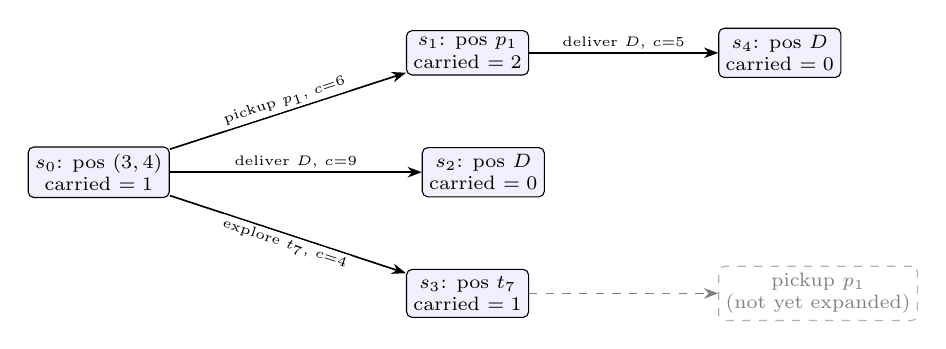
\begin{tikzpicture}[
    font=\scriptsize,
    state/.style={draw, rounded corners=2pt, align=center, inner sep=2.5pt, fill=blue!6},
    edge/.style={-{Stealth[length=1.8mm]}, semithick},
    w/.style={font=\tiny, fill=white, inner sep=1pt},
    dim/.style={draw=gray!60, dashed, rounded corners=2pt, align=center, inner sep=2.5pt, text=gray}
]
\node[state] (s0) {$s_0$: pos $(3,4)$\\carried $=1$};
\node[state, above right=9mm and 30mm of s0] (s1) {$s_1$: pos $p_1$\\carried $=2$};
\node[state, right=32mm of s0] (s2) {$s_2$: pos $D$\\carried $=0$};
\node[state, below right=9mm and 30mm of s0] (s3) {$s_3$: pos $t_7$\\carried $=1$};
\node[state, right=24mm of s1] (s4) {$s_4$: pos $D$\\carried $=0$};
\node[dim, right=24mm of s3] (s5) {pickup $p_1$\\(not yet expanded)};
\draw[edge] (s0) -- node[w, above, sloped]{pickup $p_1$, $c{=}6$} (s1);
\draw[edge] (s0) -- node[w, above]{deliver $D$, $c{=}9$} (s2);
\draw[edge] (s0) -- node[w, below, sloped]{explore $t_7$, $c{=}4$} (s3);
\draw[edge] (s1) -- node[w, above]{deliver $D$, $c{=}5$} (s4);
\draw[edge, dashed, gray] (s3) -- (s5);
\end{tikzpicture}
\caption{Fragment of the logical state-space graph. Nodes are desire-level abstractions of the
game state; edges are desires weighted by memoised A* costs $c$ and rewarded by the fuzzy
scorer. The graph is expanded lazily, only where the search visits it.}
\label{fig:stategraph}
\end{figure}

\subsection{MCTS over desire sequences}
\texttt{MCTSIntentionStrategy} runs the four canonical MCTS
phases~\cite{swiechowski2023mcts} over this graph for a fixed iteration budget
(Figure~\ref{fig:mcts}); casting the decision problem at the task level rather than the
primitive-action level follows the way MCTS is applied to scheduling problems in dynamic,
uncertain domains~\cite{norman2024satellite,liu2025fooddelivery}:

\begin{enumerate}
    \item \textbf{Selection}: from the root (the agent's real current state), descend through
    fully expanded nodes by maximising UCB1,
    $\overline{R}_i + c\sqrt{\ln N / n_i}$ with $c = \sqrt{2}$, balancing the exploitation of
    high-reward desire sequences against the exploration of rarely tried ones.
    \item \textbf{Expansion}: materialise one untried desire edge of the reached node,
    computing the child state via the transition function of Section~\ref{sec:stategraph}.
    \item \textbf{Simulation}: perform a random rollout of desires from the child down to a
    fixed maximum depth (5 logical steps); the game has no terminal state, so the rollout value
    is the accumulated fuzzy reward along the sampled sequence.
    \item \textbf{Backpropagation}: add the rollout value to the visit and reward statistics of
    every node on the path back to the root.
\end{enumerate}

The core loop is deliberately close to the textbook formulation:

\begin{lstlisting}[language=Java]
for (let i = 0; i < this.iterations; i++) {
  let node = root;
  // Selection: descend via UCB1 while fully expanded
  while (node.isFullyExpanded && node.children.length > 0
         && node.state.visited.size < this.maxDepth) {
    node = selectChild(node, this.explorationConstant);
  }
  // Expansion: materialise one untried desire edge
  if (!node.isFullyExpanded && node.state.visited.size < this.maxDepth) {
    node = await expand(node, desires, costEstimator, scorer);
  }
  // Simulation + Backpropagation
  const reward = await rollout(node.state, desires, costEstimator, scorer, this.maxDepth);
  backpropagate(node, reward);
}
\end{lstlisting}

After the budget is exhausted the strategy returns the \emph{robust
child}~\cite{swiechowski2023mcts}: the root action with the highest visit count rather than the
highest average reward, a standard choice that is less sensitive to a few lucky rollouts. Only the first desire of the best sequence is committed;
the search is re-run on the next deliberation cycle against fresh beliefs, which keeps the
lookahead honest in a dynamic, adversarial environment while the plan-level reactivity
(Section~\ref{sec:planning}) handles the execution details.

\begin{figure}[htbp]
\centering
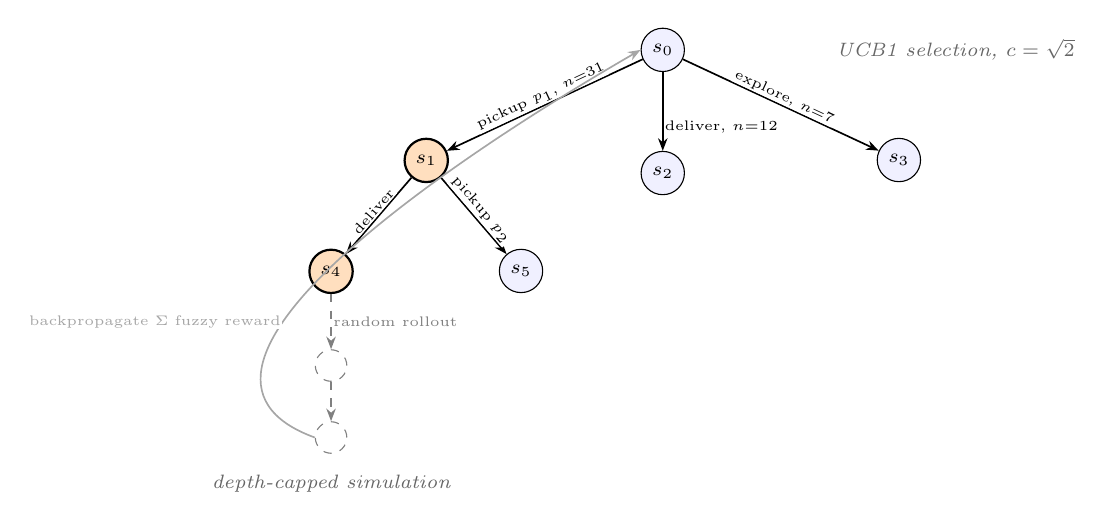
\begin{tikzpicture}[
    font=\scriptsize,
    n/.style={draw, circle, inner sep=1.5pt, minimum size=5.5mm, fill=blue!6},
    best/.style={draw, circle, inner sep=1.5pt, minimum size=5.5mm, fill=orange!25, thick},
    sim/.style={draw=gray, circle, inner sep=1pt, minimum size=4mm, dashed},
    edge/.style={-{Stealth[length=1.6mm]}, semithick},
    lab/.style={font=\tiny, fill=white, inner sep=0.5pt},
    phase/.style={font=\scriptsize\itshape, text=black!60}
]
\node[n] (root) {$s_0$};
\node[best, below left=10mm and 26mm of root] (a) {$s_1$};
\node[n, below=10mm of root] (b) {$s_2$};
\node[n, below right=10mm and 26mm of root] (c) {$s_3$};
\node[best, below left=10mm and 8mm of a] (a1) {$s_4$};
\node[n, below right=10mm and 8mm of a] (a2) {$s_5$};
\node[sim, below=7mm of a1] (r1) {};
\node[sim, below=5mm of r1] (r2) {};
\draw[edge] (root) -- node[lab, above, sloped]{pickup $p_1$, $n{=}31$} (a);
\draw[edge] (root) -- node[lab, right, pos=0.7]{deliver, $n{=}12$} (b);
\draw[edge] (root) -- node[lab, above, sloped]{explore, $n{=}7$} (c);
\draw[edge] (a) -- node[lab, above, sloped]{deliver} (a1);
\draw[edge] (a) -- node[lab, above, sloped]{pickup $p_2$} (a2);
\draw[edge, dashed, gray] (a1) -- node[lab, right]{random rollout} (r1);
\draw[edge, dashed, gray] (r1) -- (r2);
\draw[edge, gray!70] (r2.west) to[out=160, in=-150] node[lab, left, pos=0.35]{backpropagate $\Sigma$ fuzzy reward} (root.west);
\node[phase, right=18mm of root] {UCB1 selection, $c=\sqrt{2}$};
\node[phase, below=1.5mm of r2] {depth-capped simulation};
\end{tikzpicture}
\caption{One MCTS iteration over the logical state space. Highlighted nodes form the
most-visited (robust) path; the root child with the highest visit count ($s_1$, pickup $p_1$)
becomes the committed intention.}
\label{fig:mcts}
\end{figure}

\section{Fuzzy Logic as a Common Currency for Heterogeneous Metrics}
\label{sec:fuzzy}

Desire evaluations mix quantities that live on incompatible scales: traversal cost (grid steps),
expected reward (game points), and urgency (an ordinal priority). Early ad hoc utility formulas
(e.g.\ $\log(\mathit{reward})/\log(\mathit{cost}+1)$ for pickups, $-\mathit{cost}$ for
deliveries, pure staleness for exploration) were mutually incomparable, which is fatal for a
search that must rank pickups \emph{against} deliveries \emph{against} exploration. The
\texttt{FuzzyDesirabilityScorer} solves this with a Mamdani fuzzy inference system that maps
every evaluation onto a single desirability scale $[0,100]$ (Figure~\ref{fig:fuzzy}) --- the same
role fuzzy control plays in blending heterogeneous, uncertain signals in autonomous robot
navigation~\cite{saffiotti1997} and in agent-based game behaviour design~\cite{li2004fuzzy}.

\paragraph{Fuzzification with game-derived scales.} Cost and reward are fuzzified into
\textsc{low}/\textsc{medium}/\textsc{high} sets built from shoulder and triangular membership
functions. Crucially, the set breakpoints are not constants but are derived per match from the
live game configuration: cost breakpoints as fractions ($0.15$, $0.30$, $0.50$) of the
Manhattan-style upper bound $\mathit{width}+\mathit{height}$ (empirically a much better ceiling
for obstacle-laden grid traversal than the Euclidean diagonal), and reward breakpoints as
multiples ($0.3\times$, $1\times$, $1.75\times$) of the server-provided
\texttt{reward\_average}. Anchoring on the average alone (rather than
$\mu \pm \sqrt{\sigma^2}$) keeps the scale meaningful when \texttt{reward\_variance} is zero,
and lets a multi-parcel delivery (summed reward) correctly read as \textsc{high}. The scorer is
instantiated once per search, so the scale is computed once from the belief and shared across
all evaluations of that search.

\paragraph{Rule base and defuzzification.} A compact rule base combines the memberships with
$\min$ (fuzzy AND), e.g.
\emph{if cost is low and reward is high then desirability is high};
\emph{if cost is high and reward is low then desirability is low};
urgency contributes two crisp rules that pull the output toward \textsc{high} or \textsc{low}.
Rules over \emph{risk} were deliberately removed after calibration showed they fired uniformly
(no desire currently populates a non-zero risk) and only biased every score downward; they will
return once a real risk signal exists. Following Mamdani inference, each fired rule clips its
output set at its firing strength, the clipped sets are aggregated by fuzzy union, and the crisp
score is the centroid of the aggregate, sampled numerically over $[0,100]$.

This score is used uniformly across the agent: as the per-step reward inside MCTS rollouts, and
by the open-minded reconsideration policy when comparing a challenger desire against the current
commitment --- i.e.\ every comparison between options, wherever it happens, goes through the same
fuzzy currency.

\begin{figure}[htbp]
\centering
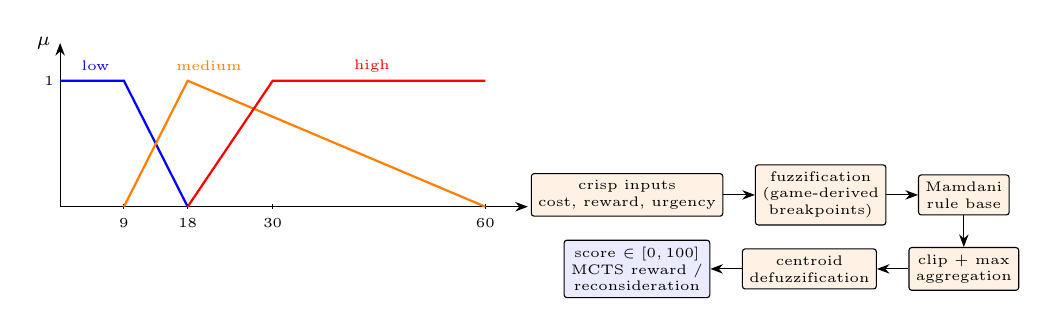
\begin{tikzpicture}[font=\scriptsize]
% hand-drawn membership plot (x: 0..60 cost -> 0..5.4cm, y: 0..1 -> 0..1.6cm)
\begin{scope}[xscale=0.09, yscale=1.6]
  \draw[-{Stealth[length=1.6mm]}] (0,0) -- (66,0) node[right]{cost};
  \draw[-{Stealth[length=1.6mm]}] (0,0) -- (0,1.3) node[left]{$\mu$};
  \foreach \x in {9,18,30,60} \draw (\x,0.02) -- (\x,-0.02) node[below]{\tiny \x};
  \draw (0.5,1) node[left]{\tiny 1};
  \draw[thick, blue]   (0,1) -- (9,1) -- (18,0);
  \draw[thick, orange] (9,0) -- (18,1) -- (60,0);
  \draw[thick, red]    (18,0) -- (30,1) -- (60,1);
  \node[blue, font=\tiny]   at (5,1.12) {low};
  \node[orange, font=\tiny] at (21,1.12) {medium};
  \node[red, font=\tiny]    at (44,1.12) {high};
\end{scope}
\begin{scope}[xshift=7.2cm, yshift=0.15cm,
    b/.style={draw, rounded corners=1pt, align=center, inner sep=2.5pt, fill=orange!10, font=\tiny},
    arr/.style={-{Stealth[length=1.6mm]}}]
\node[b] (in) {crisp inputs\\cost, reward, urgency};
\node[b, right=4mm of in] (fz) {fuzzification\\(game-derived\\breakpoints)};
\node[b, right=4mm of fz] (rules) {Mamdani\\rule base};
\node[b, below=4mm of rules] (agg) {clip + max\\aggregation};
\node[b, left=4mm of agg] (df) {centroid\\defuzzification};
\node[b, left=4mm of df, fill=blue!8] (out) {score $\in [0,100]$\\MCTS reward /\\reconsideration};
\draw[arr] (in) -- (fz);
\draw[arr] (fz) -- (rules);
\draw[arr] (rules) -- (agg);
\draw[arr] (agg) -- (df);
\draw[arr] (df) -- (out);
\end{scope}
\end{tikzpicture}
\caption{Left: cost membership functions on a $30{\times}30$ map (breakpoints at $9/18/30$
derived from $\mathit{width}+\mathit{height}=60$). Right: the Mamdani inference pipeline that
turns heterogeneous metrics into a single comparable desirability score.}
\label{fig:fuzzy}
\end{figure}

\section{Planning, PDDL, and Anytime Plan Refinement}
\label{sec:planning}

Once a desire is committed, \texttt{Planner} turns it into a concrete action plan by trying an
ordered chain of pathfinders and taking the first that succeeds:

\begin{enumerate}
    \item \textbf{A*} (\texttt{AStarPathFinder}) with Manhattan heuristic for plain navigation.
    Benchmarks (Section~\ref{sec:validation}) show it comfortably fits inside a single movement
    tick on every official map, so it is always attempted first.
    \item \textbf{PDDL} (\texttt{PDDL\_PathFinder}) for situations A* cannot express ---
    in particular maps where movable \emph{crates} block the only corridors and must be pushed
    aside, a Sokoban-style problem that is genuinely relational rather than a shortest-path
    query --- Sokoban is PSPACE-complete and a classic hard planning
    benchmark~\cite{virkkala2011,peters2023}, which makes it exactly the kind of sub-problem
    worth delegating to a planner.
\end{enumerate}

\subsection{PDDL domain and problem generation}
The domain models the agent as a \texttt{sokoban} and crates as pushable objects, with typed
\texttt{move-\{up,down,left,right\}} and \texttt{push-\{up,down,left,right\}} actions guarded by
directional adjacency predicates, tile occupancy (\texttt{free-tile}), and
\texttt{crates-allowed-tile} constraints, while a numeric fluent \texttt{total-distance}
accumulates the plan metric to be minimised. The push actions are the relational heart of the domain:

\begin{lstlisting}
(:action push-up
  :parameters (?sokoban - sokoban ?crate - crate
               ?sokobanFromTile ?crateFromTile ?crateToTile - tile)
  :precondition (and (on ?sokoban ?sokobanFromTile) (on ?crate ?crateFromTile)
                     (adjacent-up ?sokobanFromTile ?crateFromTile)
                     (adjacent-up ?crateFromTile ?crateToTile)
                     (free-tile ?crateToTile) (crates-allowed-tile ?crateToTile))
  :effect (and (free-tile ?sokobanFromTile) (not (on ?sokoban ?sokobanFromTile))
               (not (on ?crate ?crateFromTile)) (not (free-tile ?crateToTile))
               (on ?sokoban ?crateFromTile) (on ?crate ?crateToTile)
               (increase (total-distance) 1)))
\end{lstlisting}

Problems are generated on demand from the live
belief by a dedicated generator supporting two occupancy modes: \textsc{clean-map} (only static
walls and crates constrain the problem) and \textsc{frozen-snapshot} (currently sensed rival
positions are additionally frozen in as obstacles), trading optimism against congestion
awareness. Tiles are emitted as objects \texttt{tile\_x\_y} only for walkable cells, with
directional \texttt{adjacent-*} facts derived from the belief's grid, so plan steps can be
translated back to grid moves deterministically.

\subsection{Anytime planning via an extended PaaS}
Sokoban-like problems can take a satisficing planner well into seconds, but a satisficing
\emph{first} answer often arrives quickly and is then progressively improved. To exploit this,
we extended the open-source planning infrastructure at both ends (an upstream pull request is
in progress for the server side):

\begin{itemize}
    \item \textbf{Client} --- a published fork of \texttt{@unitn-asa/pddl-client}
    (\texttt{@matteoranzi/pddl-client}) whose \texttt{onlineSolver} gains
    (i)~\texttt{onImprovedPlan(plan, metric)}, a callback invoked every time an anytime planner
    (e.g.\ OPTIC) reports a better solution while still searching, rather than a single result
    at the end; (ii)~a per-request \texttt{maxTime} budget override; and (iii)~an
    \texttt{AbortSignal} that not only stops the client from waiting but instructs the server to
    kill the planner process, freeing the worker.
    \item \textbf{Server} --- a fork of AI-Planning \texttt{planning-as-a-service}
    (branch \texttt{feat/stream-anytime-progress}) that streams intermediate plans to the client
    instead of buffering until the solver exits.
\end{itemize}

The agent uses these primitives to bound planning latency: as soon as the first improved plan
arrives, the solve is aborted and the plan executed, capping worst-case waiting at the
configured budget while still benefiting from any early improvement:

\begin{lstlisting}[language=Java]
const finalPlan = await onlineSolver(this.domainText, problem.toPddlString(), {
  maxTime: this.maxSolvingTimeS,
  signal: controller.signal,
  onImprovedPlan: (improvedPlan, metric) => {
    plan = improvedPlan;   // best plan streamed by the anytime planner so far
    controller.abort();    // good enough: stop the solver, start executing
  },
});
plan ??= finalPlan;
\end{lstlisting} The same machinery is the
substrate for a planned refinement --- hot-swapping the executing plan whenever the anytime
planner later finds a strictly cheaper one, re-anchored to the agent's current position
(Section~\ref{sec:future}).

\subsection{Plan execution and failure recovery}
\texttt{PlanExecutor} executes plans one action at a time, re-checking before every step that
the committed desire is still valid and still committed --- so an intention switch or a belief
change aborts the plan at the next step boundary, in classic BDI style. Failed actions
(typically a rival occupying the next tile) are handled by composable recovery strategies
implementing an escalation chain, e.g.\ \emph{retry $n$ times} $\rightarrow$ \emph{replan from
the current position (up to $m$ times)} $\rightarrow$ \emph{abort and re-deliberate}. The
strategy object is created fresh per execution, keeping retry budgets per-plan, and the
decorator-style composition (\texttt{ReplanThenAbort} wrapping \texttt{RetryThenAbort}) makes
persistence policies declarative and swappable.

\section{LLM-Controlled Agent}
\label{sec:llm}

The LLM-controlled agent (Agent B) uses a local Large Language Model to transform
natural-language requests into structured Deliveroo.js actions. It combines an autonomous
fallback policy with an interactive chat interface: when no request is pending the agent behaves
autonomously; when a user message arrives, the LLM temporarily takes responsibility for
high-level planning. The LLM never receives unrestricted control: it returns a strict JSON
object containing a textual response and a plan composed only of supported tools, conditions,
and bounded loops, which the local application parses and executes.

\subsection{Architecture and execution flow}
The main component, \texttt{LlmAgent.js}, manages the Deliveroo.js connection, local world
state (\texttt{WorldModel.js}: map, agent position, visible parcels, delivery and spawning
tiles), autonomous behaviour, user requests, and LLM plan execution. When a chat request is
received: the request is queued; the agent enters \texttt{LLM\_MODE}, pausing autonomous
decisions (avoiding the autonomous policy and the LLM plan steering the agent toward different
targets); \texttt{promptBuilder.js} combines the user message, a compact world snapshot, and
persistent memory (\texttt{memory.txt}, storing learned facts, reward observations, and
strategy rules); \texttt{ollama.js} queries a local Ollama model; \texttt{parser.js} interprets
and executes the returned plan; finally the agent resumes its fallback policy. A guard prevents
concurrent request processing. Figure~\ref{fig:llm-pipeline} summarises this pipeline.

\begin{figure}[htbp]
    \centering
    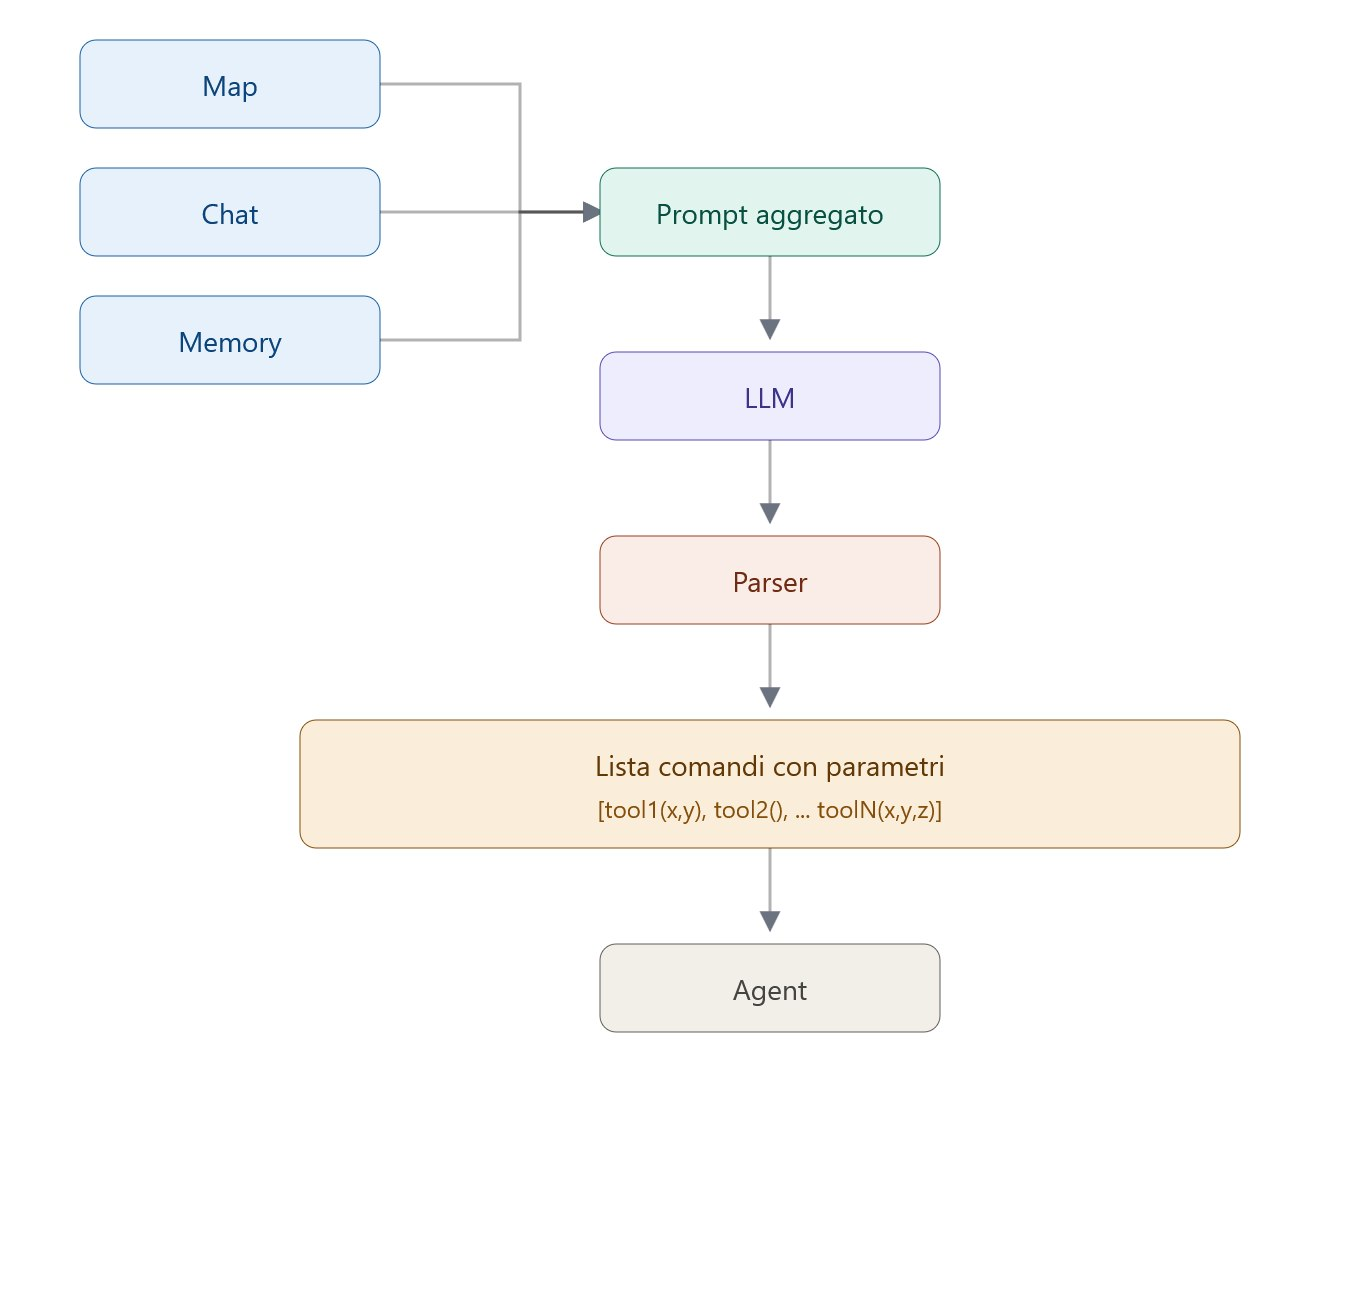
\includegraphics[width=0.56\linewidth, trim={50 250 90 20}, clip]{figures/llm_pipeline.jpg}
    \caption{LLM-controlled agent pipeline. The map state, chat request, and persistent memory
    are aggregated into a single prompt; the LLM output is parsed into a parameterised command
    list (\texttt{tool$_1$(x,y)}, \dots, \texttt{tool$_N$(x,y,z)}), which is then executed by
    the agent.}
    \label{fig:llm-pipeline}
\end{figure}

Outside \texttt{LLM\_MODE}, the fallback strategy prioritises on-tile actions (pickup,
delivery), then targets: deliver when carrying many parcels, move toward the nearest reachable
free parcel, deliver when carrying with no visible parcel, otherwise explore. Navigation uses
A* with visible agents treated as temporary obstacles, moving one step at a time so the world
state refreshes between movements.

\subsection{Constrained plan interpreter and tools}
The LLM must return JSON only, with a \texttt{chat} field shown to the user and a \texttt{plan}
field: a small domain-specific language of direct tool calls,
\texttt{if}/\texttt{then}/\texttt{else} branches, and condition-guarded \texttt{loop} blocks ---
never arbitrary code. Tool names resolve through a predefined mapping, so the LLM can invoke
only intentionally exposed functions: \texttt{move\_to} (A* navigation with step limits),
\texttt{pick\_up\_parcel} / \texttt{put\_down\_parcel}, \texttt{find\_and\_get\_a\_parcel} (a
reactive search that refreshes its target after each movement, handling parcels that expire or
are taken by rivals), \texttt{calculator}, \texttt{add\_to\_memory}, and
\texttt{reply\_to\_server}. The interpreter applies defensive limits --- bounded loop iterations,
abort after repeated failed iterations, termination on fatal movement or network errors ---
because generated plans may be incomplete or based on outdated observations.

\subsection{MCP-based control of a second agent}
The system can coordinate a separate agent (\texttt{BdiLlmTestAgent.js}) through the Model
Context Protocol: the second agent runs independently, connects to Deliveroo.js, and exposes
selected capabilities via an HTTP MCP endpoint. The LLM agent drives it through explicit typed
proxy tools (\texttt{agent\_move\_to}, \texttt{agent\_pick\_up\_parcel},
\texttt{agent\_put\_down\_parcel}, \texttt{agent\_find\_and\_get\_a\_parcel},
\texttt{agent\_get\_state}), refreshing its state before evaluating conditions that involve it.
This provides process separation: the LLM cannot touch the remote agent's internals, only a
restricted, typed action interface.

\subsection{Web interface}
The \texttt{webchat.js} component provides a browser chat panel with plan visualisation,
receiving messages over HTTP and streaming replies via Server-Sent Events.
Figure~\ref{fig:webchat-example} shows a request mixing an informational question with a
movement task; the LLM answers the question and emits four explicit \texttt{move\_to} actions.
More complex plans combine bounded local collection loops, delivery actions, and remote MCP
commands for the second agent.

\begin{figure}[htbp]
    \centering
    \begin{minipage}[c]{0.66\linewidth}
        \centering
        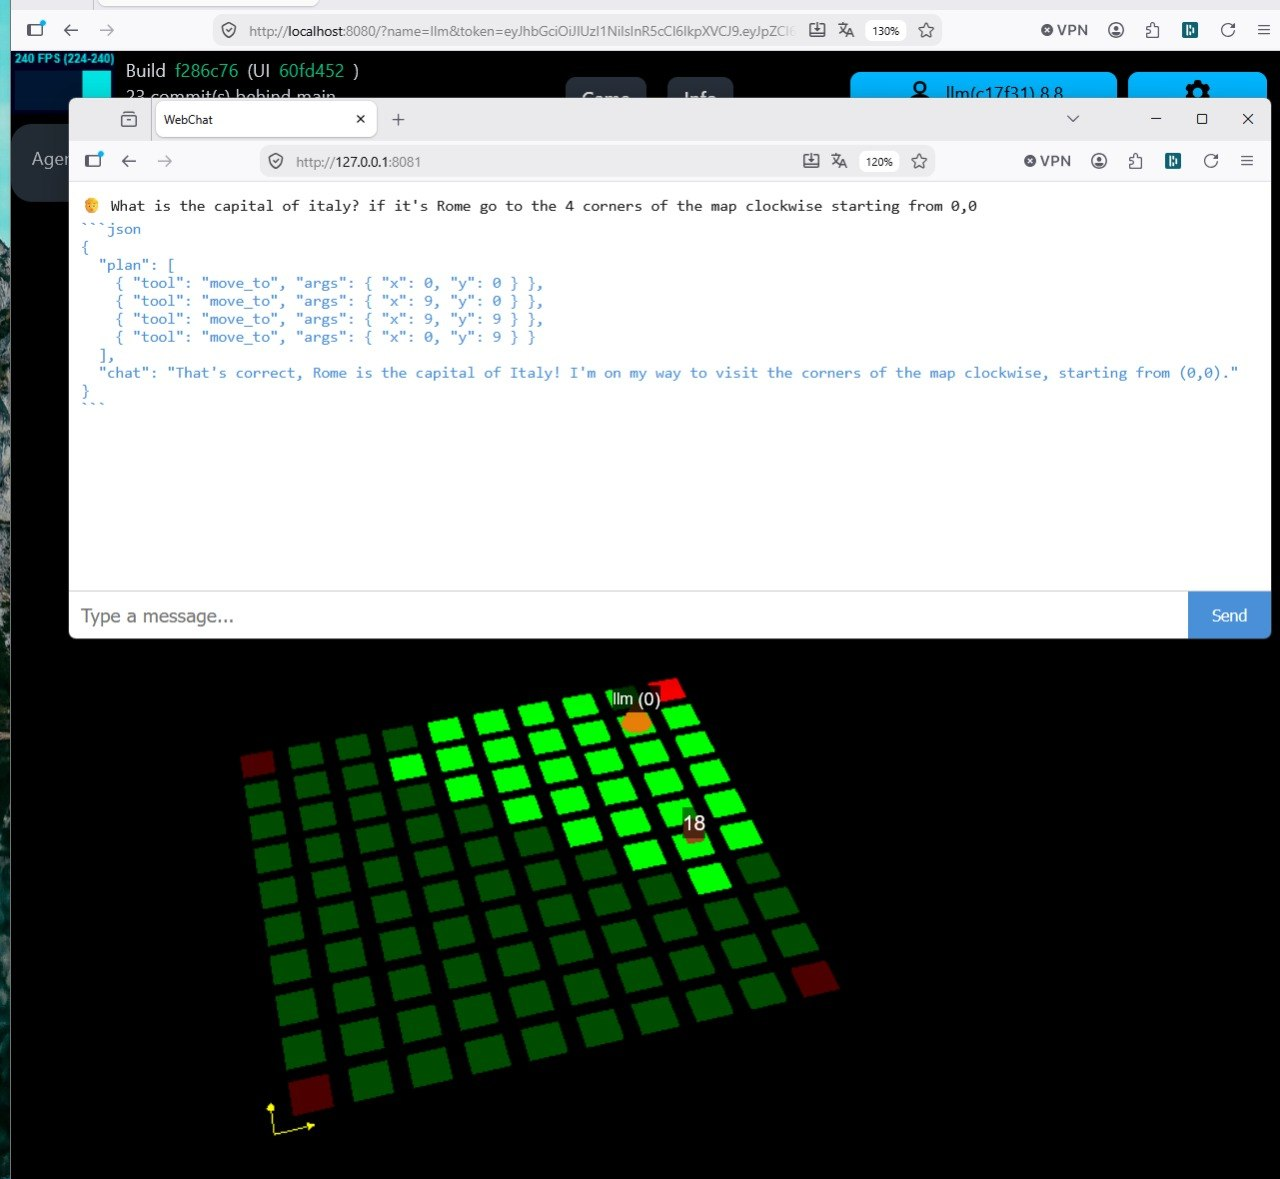
\includegraphics[width=\linewidth]{figures/webchat_example.jpg}
    \end{minipage}\hfill
    \begin{minipage}[c]{0.30\linewidth}
        \centering
        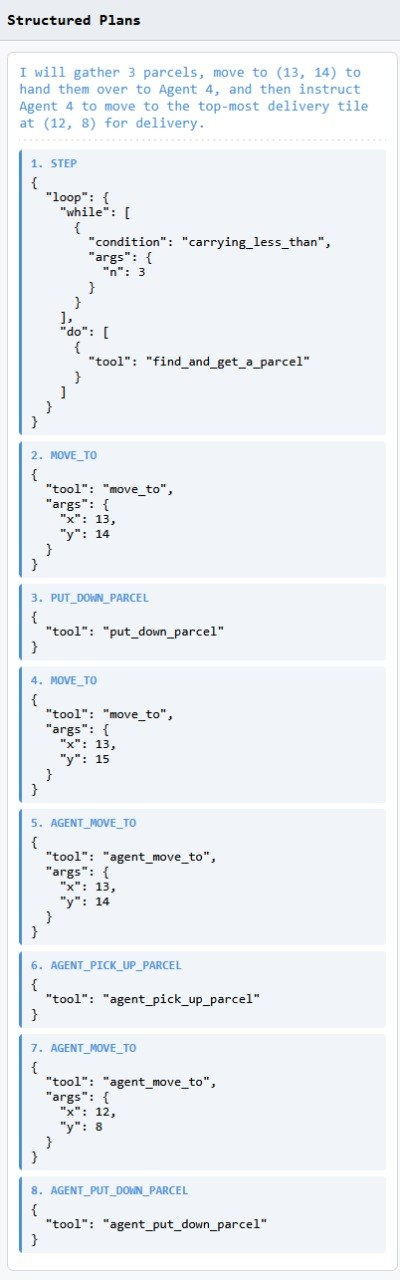
\includegraphics[height=7.8cm,keepaspectratio]{figures/complex_plan.jpg}
    \end{minipage}
    \caption{Left: web-chat example --- the agent answers a natural-language request and
    generates a JSON plan with four coordinate-based movement actions. Right: a multi-step plan
    combining a bounded local collection loop, delivery actions, and remote MCP commands that
    direct the second agent to collect and deliver a hand-over parcel.}
    \label{fig:webchat-example}
\end{figure}

\section{Validation and Calibration}
\label{sec:validation}

\paragraph{Pathfinding benchmarks.} A* was benchmarked on the official challenge maps by
computing, from a random start, the path to every valid tile, averaged over 300 iterations per
map (MacBook Pro M1 Max):

\begin{table}[htbp]
\centering
\footnotesize
\begin{tabular}{lrr}
\toprule
Map & Time (ms) & Valid tiles \\
\midrule
\texttt{empty\_30} & 21.45 & 900 \\
\texttt{circuit\_directional} & 16.20 & 485 \\
\texttt{hallways\_interconnected} & 8.56 & 465 \\
\texttt{caothic\_maze} & 7.16 & 432 \\
\texttt{wide\_path} & 12.14 & 526 \\
\texttt{two\_obstacles} & 11.36 & 524 \\
\texttt{crates\_one\_way} & 0.31 & 47 \\
\bottomrule
\end{tabular}
\caption{A* pathfinding: total time to reach every valid tile from a random start. With move
durations of at least 50\,ms, planning always fits well within a single movement tick.}
\label{tab:astar}
\end{table}

\paragraph{Data-driven fuzzy/MCTS calibration.} Rather than hand-guessing constants, the live
agent was instrumented: a one-time dump of the server-provided game configuration, a periodic
\texttt{[FUZZY-CALIBRATE]} log recording observed min/max cost, reward, and score per desire
category against the active fuzzy scale, and a per-search \texttt{[MCTS-CALIBRATE]} log
recording root branching factor, total visits, and the top visited children. This surfaced and
fixed several concrete issues: cost breakpoints moved from the Euclidean diagonal (real A* costs
reached 58 on a $30{\times}30$ map, past $\sqrt{w^2+h^2}\approx 42$) to $w+h$; reward
breakpoints were made robust to zero-variance reward distributions; delivery and exploration
desires that silently reported a zero reward signal were repaired; and dead risk rules were
removed. On the MCTS side, calibration revealed that the effective bottleneck was not the UCB1
constant but the root branching factor (57--95 children, dominated by per-spawner exploration
desires): with 100 iterations, UCB1's forced first visit to every child consumed most of the
budget, and visit concentration improved sharply whenever branching dropped. This motivates the
exploration-desire aggregation discussed in Section~\ref{sec:future}.

\paragraph{Scenario testing and observability.} The BDI agent was validated on the Challenge~1
scenario maps (including the crate-blocked \texttt{crates\_one\_way} map exercising the PDDL
pathfinder), and the LLM agent on Challenge~2 atomic-request scenarios through the chat
interface. A live terminal UI (Figure~\ref{fig:bdi-log}) renders the full deliberation state ---
belief grid, current desire set with evaluations, the change-detection strategies that triggered
the last cycle, and the committed intention with its fuzzy score --- which proved essential both
for debugging emergent behaviour and for the calibration campaign above.

\begin{figure}[htbp]
    \centering
    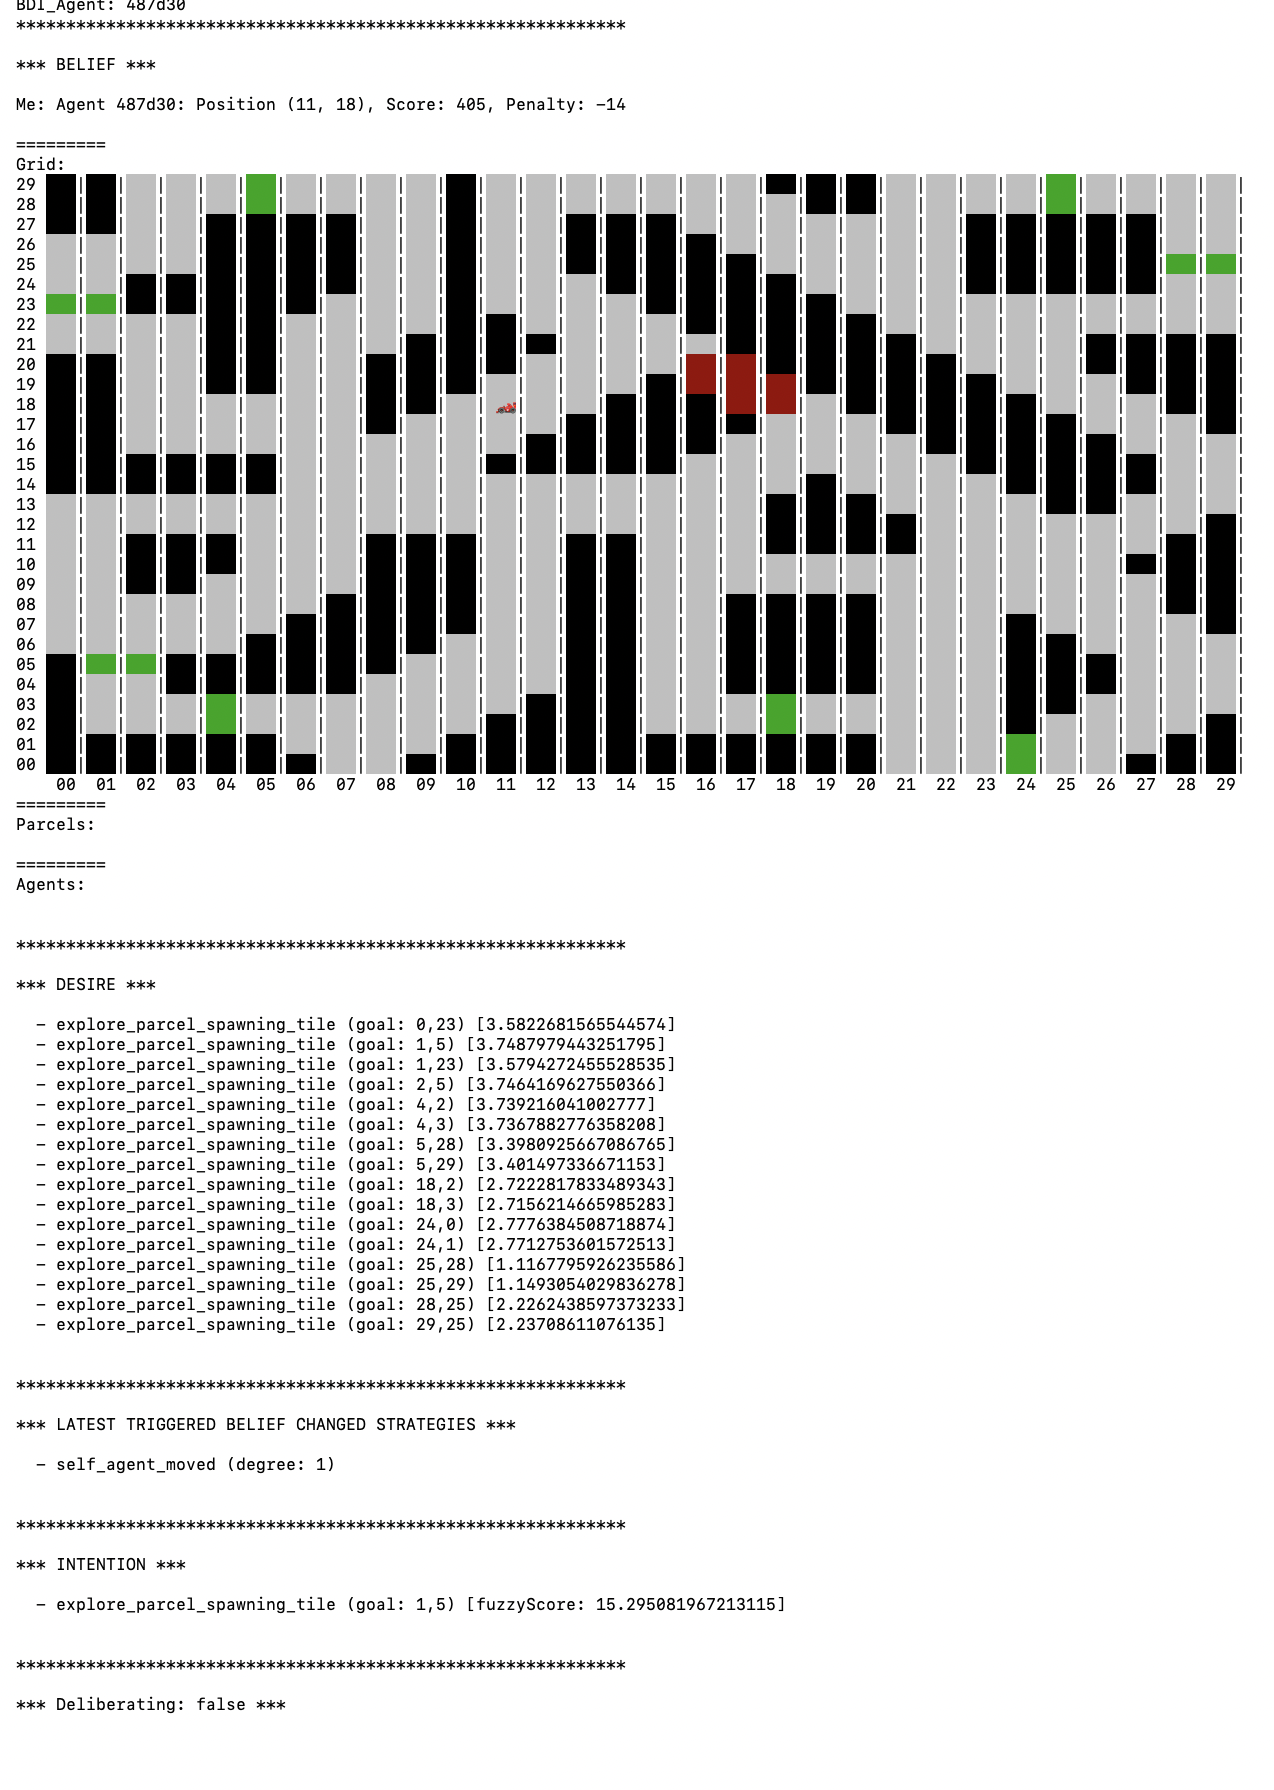
\includegraphics[height=12.6cm,keepaspectratio]{figures/bdi_log.png}
    \caption{Live terminal UI of the BDI agent on a $30{\times}30$ map: belief grid (agent,
    walls, spawner and delivery tiles), the generated exploration desires with their staleness
    evaluations, the change-detection strategies fired on the last belief update, and the
    committed intention annotated with its fuzzy desirability score.}
    \label{fig:bdi-log}
\end{figure}

\section{Conclusion and Future Development}
\label{sec:future}

The project delivers a BDI agent whose deliberation is genuinely modular --- event-driven belief
revision, desire-level MCTS lookahead over a lazily built logical state space, fuzzy inference
as a common scoring currency, and a layered A*/anytime-PDDL planning stack with composable
failure recovery --- alongside an LLM-controlled agent with a safety-constrained plan
interpreter and MCP-based control of a second agent. The interfaces introduced everywhere
(selection strategies, reconsideration policies, pathfinders, recovery strategies,
change-detection strategies) were a deliberate investment: each of the extensions below slots
into an existing seam without touching the deliberation loop.

\subsection{Future development}

\begin{itemize}
    \item \textbf{Hot-swappable intention strategies with online-tuned parameters.} Start each
    match with \texttt{GreedyIntentionStrategy} --- cheap, reactive, and insensitive to branching
    factor --- as a warm-up phase whose real purpose is data collection: observed cost and reward
    ranges per desire category, effective branching factors, and map-specific traversal
    statistics. Once enough evidence accumulates, a wrapper strategy hot-swaps to
    \texttt{MCTSIntentionStrategy} (and to a matching commitment policy) whose fuzzy breakpoints
    and search budget are calibrated from the collected statistics instead of configuration
    heuristics --- automating online the manual run--log--tune loop used in
    Section~\ref{sec:validation}. Because both strategies implement
    \texttt{IIntentionStrategy}, the swap is invisible to \texttt{Intention}.
    \item \textbf{Anytime plan hot-swapping during execution.} Extend the anytime PDDL
    integration so that improved plans arriving \emph{while a plan is executing} are adapted to
    the agent's current position and swapped in when strictly cheaper, rather than only bounding
    the initial solve.
    \item \textbf{Smarter exploration desires.} Replace per-spawner exploration desires with a
    small set of \emph{observation hotspots} computed by a greedy maximum-coverage algorithm
    over the spawner set, simultaneously improving exploration quality and collapsing the MCTS
    root branching factor identified as the main search bottleneck.
    \item \textbf{Inter-agent coordination.} Implement message-based coordination between the
    BDI and LLM agents over the Deliveroo.js communication API --- handshake and role assignment,
    periodic belief sharing (parcels and rivals seen outside the teammate's sensing range), and
    parcel reservation to avoid targeting the same parcel; even minimal local communication is
    known to yield strongly coordinated multi-agent navigation~\cite{hildreth2019}. In the same
    step, route in-game messages from the mission agent into the LLM agent's request queue, so
    that mission-agent requests are handled through the same constrained planning pipeline as
    chat requests.
    \item \textbf{Automated comparative benchmarks.} Extend the benchmark harness beyond
    pathfinding to full-match comparisons (Greedy vs.\ MCTS intention selection, A*-only vs.\
    A*+PDDL) with automated runs and result export across the challenge maps.
    \item \textbf{Risk as a live signal.} Populate the currently unused risk input of the fuzzy
    scorer from rival trajectory predictions (the belief base already tracks position
    histories), re-enabling the risk rule family removed during calibration.
    \item \textbf{Structured LLM memory.} Replace the plain-text persistent memory with a
    validated, structured store.
\end{itemize}


\begin{footnotesize}
\begin{thebibliography}{9}

\bibitem{bratman1987}
M.~E. Bratman.
\newblock \emph{Intention, Plans, and Practical Reason}.
\newblock Harvard University Press, 1987.

\bibitem{swiechowski2023mcts}
M.~Świechowski, K.~Godlewski, B.~Sawicki, and J.~Mańdziuk.
\newblock Monte Carlo Tree Search: a review of recent modifications and applications.
\newblock \emph{Artificial Intelligence Review}, 56:2497--2562, 2023.

\bibitem{norman2024satellite}
J.~Norman and F.~Rivest.
\newblock Monte Carlo Tree Search satellite scheduling under cloud cover uncertainty.
\newblock \emph{arXiv:2405.20951}, 2024.

\bibitem{liu2025fooddelivery}
L.~Liu, S.~Chen, H.~Jin, X.~Deng, Y.~Liu, and Y.~Lin.
\newblock Optimizing on-demand food delivery with BDI-based multi-agent systems and Monte Carlo
tree search scheduling.
\newblock \emph{Scientific Reports}, 15:25083, 2025.

\bibitem{caillou2015}
P.~Caillou, B.~Gaudou, A.~Grignard, C.~Q. Truong, and P.~Taillandier.
\newblock A simple-to-use BDI architecture for agent-based modeling and simulation.
\newblock In \emph{Proc.\ of the 11th Conference of the European Social Simulation Association
(ESSA)}, 2015.

\bibitem{traldi2022}
A.~Traldi, F.~Bruschetti, M.~Robol, D.~Calvaresi, M.~Roveri, and P.~Giorgini.
\newblock Real-time BDI agents: a model and its implementation.
\newblock \emph{arXiv:2205.00979}, 2022.

\bibitem{saffiotti1997}
A.~Saffiotti.
\newblock The uses of fuzzy logic in autonomous robot navigation.
\newblock \emph{Soft Computing}, 1(4):180--197, 1997.

\bibitem{li2004fuzzy}
Y.~Li, P.~Musilek, and L.~Wyard-Scott.
\newblock Fuzzy logic in agent-based game design.
\newblock In \emph{Proc.\ of the Annual Meeting of the North American Fuzzy Information
Processing Society (NAFIPS)}, 2004.

\bibitem{virkkala2011}
T.~Virkkala.
\newblock \emph{Solving Sokoban}.
\newblock Master's thesis, University of Helsinki, 2011.

\bibitem{peters2023}
N.~S. Peters.
\newblock \emph{Solving Sokoban Efficiently: Search Tree Pruning Techniques and Other
Enhancements}.
\newblock Bachelor's thesis, Technische Universität Berlin, 2023.

\bibitem{hildreth2019}
D.~Hildreth and S.~J. Guy.
\newblock Coordinating multi-agent navigation by learning communication.
\newblock \emph{Proc.\ ACM on Computer Graphics and Interactive Techniques}, 2(2), 2019.

\end{thebibliography}
\end{footnotesize}

\clearpage
\appendix
\section*{Appendix: PDDL pathfinding problem file}
\label{sec:appendix}

A complete (small) instance produced by the problem generator of
Section~\ref{sec:planning}, corresponding to a $5{\times}4$ map fragment in which a crate blocks
the only corridor to the goal; repetitive tile and adjacency declarations are elided with
\texttt{[...]}.

\begin{lstlisting}
;; problem file: deliveroo-pathfinding (generated from the live Belief)
(define (problem deliveroo-pathfinding)
(:domain default)
(:objects
    player - sokoban
    crate1 - crate
    ; tiles named tile_<x>_<y>; only walkable cells become objects
    tile_0_0 tile_1_0 tile_3_0
    tile_0_1 tile_2_1 tile_3_1 tile_4_1
    tile_0_2 tile_1_2 tile_3_2 tile_4_2
    tile_0_3 tile_1_3 tile_2_3 tile_3_3 - tile
)
; ================================================
; MAP (bottom-left origin, x rightward, y upward)
;   3    f    f    f    f     .
;   2    f    f    .    C|ac  f
;   1    f    .    ac   ac    f
;   0    A    f    .    O     .
;  y/x   0    1    2    3     4
; f: free-tile          ac: crates-allowed-tile
; C: crate (tile_3_2)   A: agent start   O: goal
; .: hole (no tile object, no adjacency)
; ================================================
(:init
    (on player tile_0_0)
    (on crate1 tile_3_2)
    ; crates-allowed tiles (static)
    (crates-allowed-tile tile_3_2)
    (crates-allowed-tile tile_2_1)
    (crates-allowed-tile tile_3_1)
    ; free tiles (walkable and currently unoccupied)
    (free-tile tile_1_0)
    (free-tile tile_3_0)
    (free-tile tile_0_1)
    [...]
    (free-tile tile_3_3)
    ; directional adjacency between walkable tiles only
    (adjacent-up tile_0_0 tile_0_1)
    (adjacent-down tile_0_1 tile_0_0)
    (adjacent-up tile_3_1 tile_3_2)
    (adjacent-down tile_3_2 tile_3_1)
    [...]
    (adjacent-right tile_2_3 tile_3_3)
    (adjacent-left tile_3_3 tile_2_3)
)
(:goal (on player tile_3_0))
(:metric minimize (total-distance))
)
\end{lstlisting}

The only plan reaching \texttt{tile\_3\_0} must walk around via row~3, \texttt{push-down} the
crate from \texttt{tile\_3\_2} to \texttt{tile\_3\_1}, come around through column~4, and
\texttt{push-left} it aside onto the \texttt{crates-allowed} tile \texttt{tile\_2\_1} before
finally descending the freed corridor --- exactly the class of paths the A* pathfinder cannot
produce.


\end{document}
